%! TEX root = ../main.tex
% =============================================================
% IMMUTABLE — generated automatically, do not edit this block
%   script          : analysis_scratch/t_cross_figure.py
%   plot_type       : t_cross
%   chapter         : 05
%   subfigures      : ch05_t_cross_10V, ch05_t_cross_20V, ch05_t_cross_30V
% =============================================================
\begin{figure}[htbp]
  \centering
  \begin{subfigure}[b]{0.32\linewidth}
    \centering
    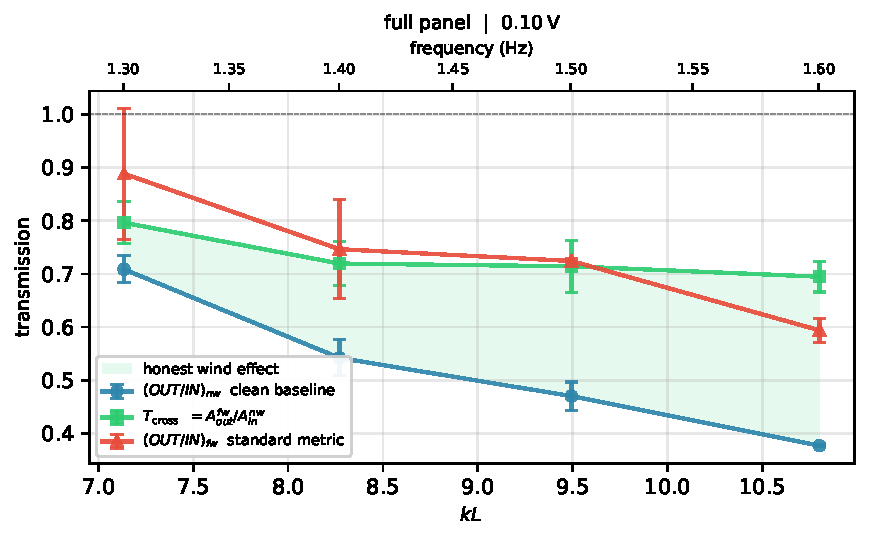
\includegraphics[width=\linewidth]{FIGURES/ch05_t_cross_10V.pdf}
    \caption{$0.10$\,V}
    \label{fig:ch05_t_cross_10V}
  \end{subfigure}
  \hfill
  \begin{subfigure}[b]{0.32\linewidth}
    \centering
    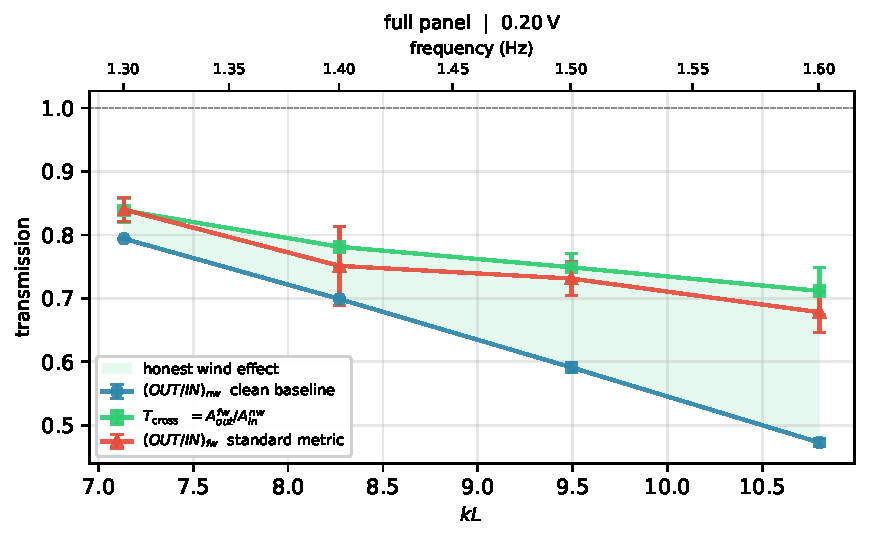
\includegraphics[width=\linewidth]{FIGURES/ch05_t_cross_20V.pdf}
    \caption{$0.20$\,V}
    \label{fig:ch05_t_cross_20V}
  \end{subfigure}
  \hfill
  \begin{subfigure}[b]{0.32\linewidth}
    \centering
    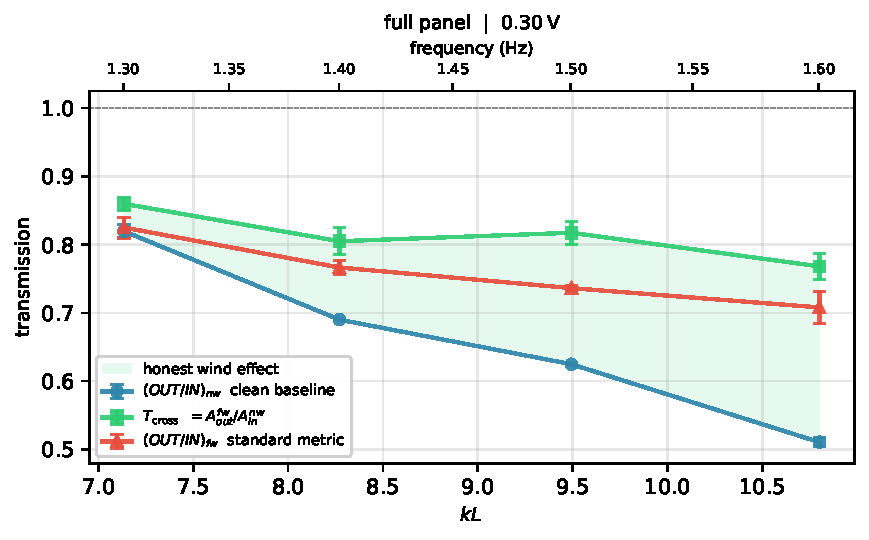
\includegraphics[width=\linewidth]{FIGURES/ch05_t_cross_30V.pdf}
    \caption{$0.30$\,V}
    \label{fig:ch05_t_cross_30V}
  \end{subfigure}
  \caption[T\_cross: wind effect via clean nowind reference]{%
    Wind effect on transmission measured three ways: $(OUT/IN)_{nw}$ (blue, nowind baseline); $T_{\mathrm{cross}} = A_{out}^{fw}/A_{in}^{nw}$ (green, fullwind OUT referenced to the clean nowind IN); and $(OUT/IN)_{fw}$ (red, standard fullwind metric). The green--blue gap is the wind effect measured with the clean incident reference. The red--blue gap is the same effect as reported by the standard ratio; the two disagree where the IN probe is contaminated by wind noise at the paddle frequency (CLAUDE.md \S 16). Worst-case divergence between the two metrics: 0.695 vs 0.594 at $f = 1.6$\,Hz, $0.10$\,V. Each subfigure is one input amplitude; $n$ per point in \texttt{analysis\_scratch/t\_cross\_figure\_summary.csv}.
  }
  \label{fig:ch05_t_cross}
\end{figure}
